
\usetikzlibrary{shadows}
\usetikzlibrary{automata, positioning, arrows, calc}
      \definecolor{falured}{rgb}{0.5, 0.09, 0.09}
     \newcommand{\fmbtsymbex}[1]{\textcolor{falured}{ #1}}
     \newcommand{\fmbtsymbexReg}[1]{ \textcolor{falured}{ #1} }
     \definecolor{mycolorData}{rgb}{0.07, 0.04, 0.56}


      \definecolor{mycolorF}{rgb}{0.973, 0.882, 0.882} 
     \definecolor{mycolorP}{rgb}{0.902, 0.957, 0.918}
     \definecolor{mycolorI}{rgb}{1.000, 0.969, 0.800}


\tikzset{
	%->,  % makes the edges directed
	%>=stealth, 
	% makes the arrow heads bold
	shorten >=2pt, shorten <=2pt, % shorten the arrow
	node distance=3cm, % specifies the minimum distance between two nodes. Change if n
	every state/.style={draw=blue!55,very thick,fill=blue!20}, % sets the properties for each ’state’ n
	initial text=$ $, % sets the text that appears on the start arrow
	%node distance=2.5cm,
    %every edge/.style={draw, bend left=20, ->}
    circled node/.style={rectangle,draw, inner sep=0, minimum size=1.5em},
    better circled node/.style={circled node,text height=.8em,text depth=.25em},
    }
\renewcommand{\arraystretch}{0.9}

%\newcommand{\myhash}{\raisebox{\depth}{\scalebox{0.8}{\#}}}
\newcommand{\myhash}{\raisebox{\depth}{\scalebox{0.8}{\text{\#}}}} 
\newcommand{\mydollar}{\raisebox{\depth}{\scalebox{0.8}{\$}}} 

	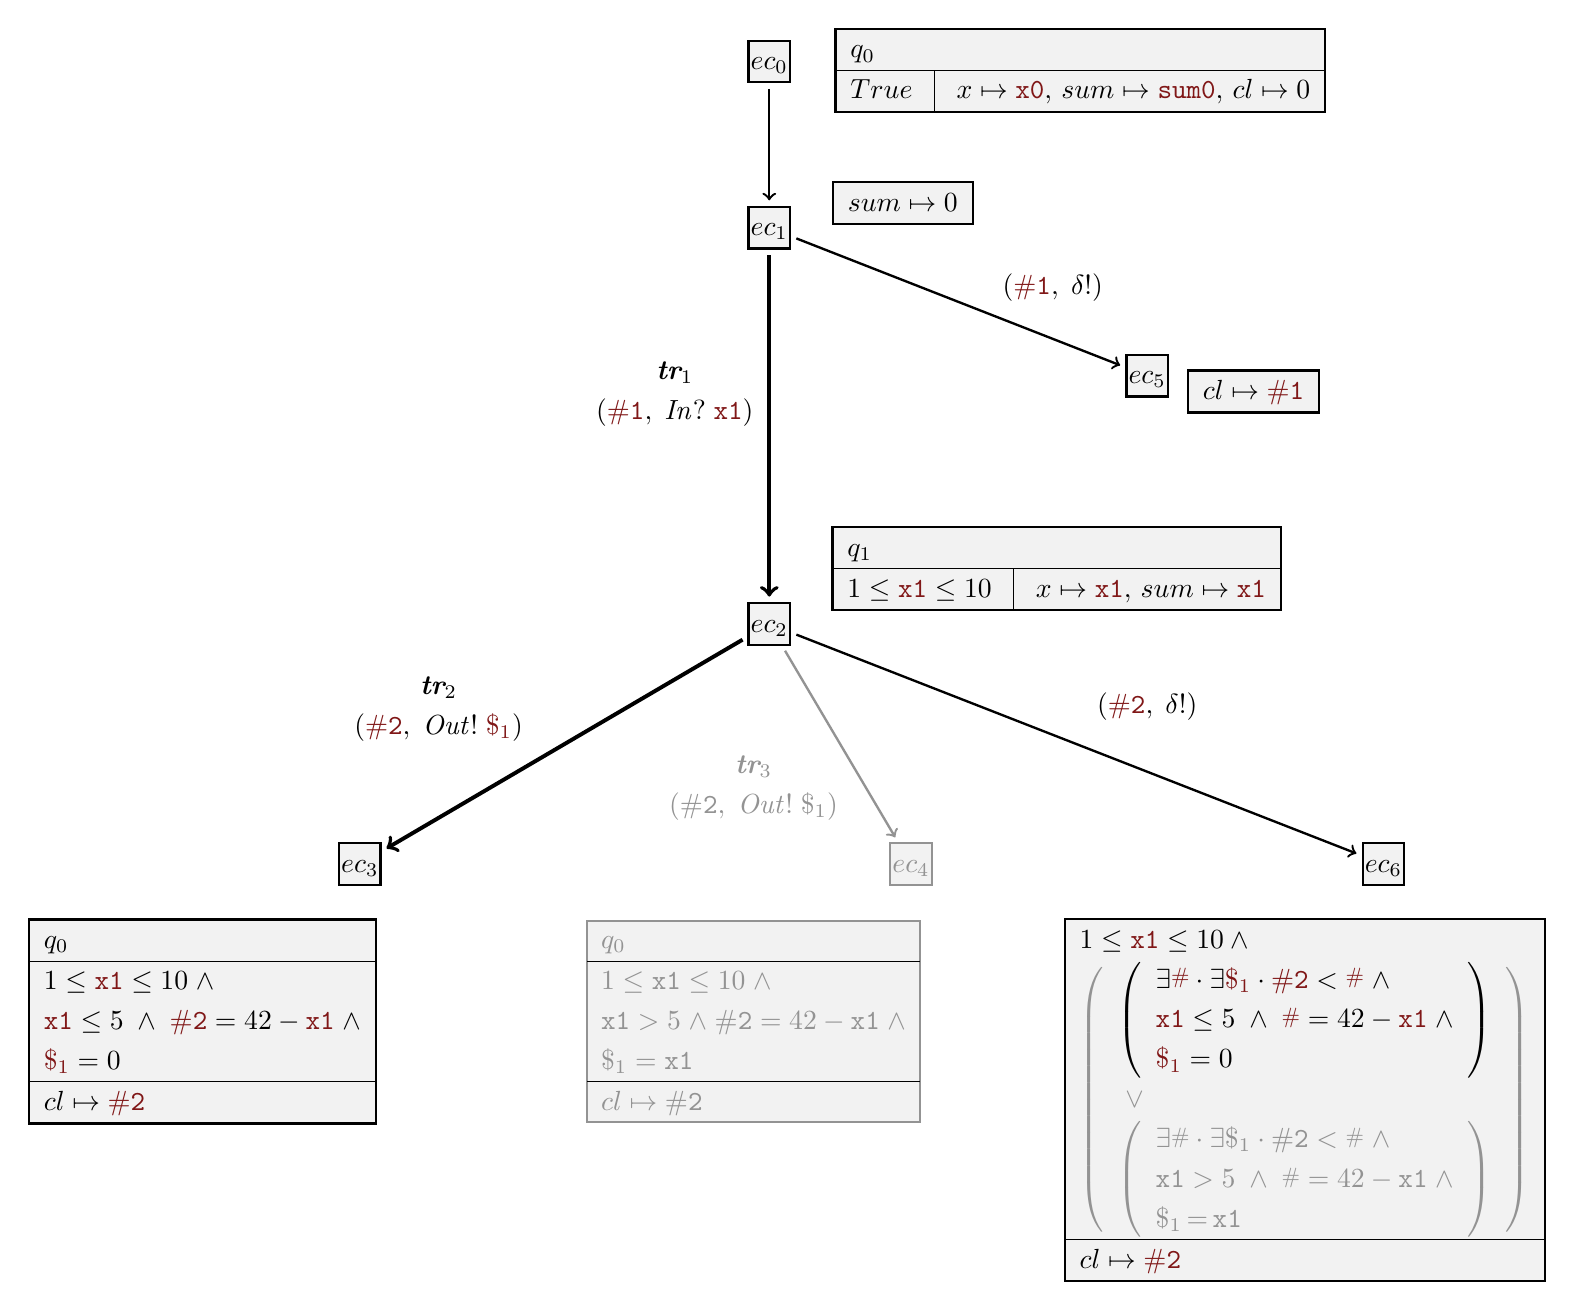
\begin{tikzpicture}
    [xscale=2, yscale=2%,font=\small %footnotesize
    ] 
	%\draw[fill=gray!20, draw=none]  (2,21.1) rectangle (10.1,15);
%\draw[fill=gray!20, draw=none]  (10.1,11.7) rectangle (-3.3,15.6);

%	\coordinate (v17) at (3,20.7) {} {};
% \draw[line width=0.3mm,draw=mycolorData,drop shadow={fill=mycolorData},fill=white] (v17) 
%     -- (11,20.7)
%     -- (11,12.328)
%     -- (-3.4,12.328)
%     -- (-3.4,15.8)
%     -- (3,15.8)
%     -- cycle;
	%\draw[line width=0.3mm,draw=black,fill=white]  (-2.92,19.972) rectangle (2.612,15.764);
	


% \draw[draw=mycolorP, line width=1.5mm]  (0.04,18.608) -- (0.04,17.0328);
% \draw[draw=mycolorP, line width=1.5mm, bend left=20]   (-0.104,16.9328)edge (-0.152,18.6094) ;
% \draw[draw=mycolorP, line width=1.5mm,dotted] (3.6,19.3029) -- (3.6,18.82);
% \draw[draw=mycolorP, line width=1.5mm,dotted] (-0.804,19.047) -- (-0.304,19.047);
% \draw[draw=mycolorP, line width=1.5mm] (3.6,18.116) -- (3.6,16.424);
% \draw[draw=mycolorP, line width=1.5mm] (3.312,15.8734) -- (0.74,14.651);
% \draw[draw=mycolorP, line width=1.5mm] (-0.168,10.3144) -- (3.276,10.3144);
% \draw[draw=mycolorP, line width=1.5mm] (4.076,10.3144) -- (7.288,10.3144);


		%\node at (4,17.784) {$\textbf{\em tr}_1$};
%\node at (0.9,15.4) {$\textbf{\em tr}_2$};

	
	
	\node[inner sep=0.0pt,fill=gray!10,line width=.3mm,draw] (v8) at (4.448,18.696) {$
	\def\arraystretch{1.2} 
\begin{array}{|l|}

\hline
sum\mapsto  0
\\
\hline
\end{array}
$};
	
	\node[circled node,line width=.3mm,fill=gray!10] (v1) at (3.6,18.54) {$\!\!\!\!
\begin{array}{c}
ec_1 
\end{array}\!\!\!\!
$};

	\node[circled node,line width=.3mm,fill=gray!10] (v4) at (3.6,19.596) {$\!\!\!\!
\begin{array}{c}
ec_0
\end{array}\!\!\!\!
$};

	\node[inner sep=0.0pt,fill=gray!10,line width=.3mm,draw] (v7) at (5.575,19.54) {$
	\def\arraystretch{1.2} 
\begin{array}{|l|l|}
\hline
\multicolumn{2}{|l|}{q_0}
\\
\hline
True \;&\; x \mapsto \fmbtsymbexReg{\mathtt{x0}},\,sum\mapsto  \fmbtsymbexReg{\mathtt{sum0}},\,cl \mapsto 0 \\
\hline
\end{array}
$};
		


\node[circled node,line width=.3mm,fill=gray!10] (v2) at (3.6,16.024) {$\!\!\!\!
\begin{array}{c}
ec_2 
\end{array}\!\!\!\!
$};

	\node[inner sep=0.0pt,fill=gray!10,line width=.3mm,draw] (v10) at (5.425,16.375) {$
	\def\arraystretch{1.2} 
\begin{array}{|l|l|}
\hline
\multicolumn{2}{|l|}{q_1}
\\
\hline
1 \le \fmbtsymbexReg{\mathtt{x1}} \le 10
\;&\;
x \mapsto \fmbtsymbexReg{\mathtt{x1}},\,
sum \mapsto \fmbtsymbexReg{\mathtt{x1}}
\\
\hline
\end{array}
$};
	\node[inner sep=0.0pt,fill=gray!10,line width=.3mm,draw] (v12) at (6.675,17.5) {$
	\def\arraystretch{1.2} 
\begin{array}{|l|}
\hline
cl \mapsto \fmbtsymbex{\mathtt{\#1}}
\\
\hline
\end{array}
$};


	\node[inner sep=0.0pt,fill=gray!10,line width=.3mm,draw] (v11) at (0,13.5) {
	$ \def\arraystretch{1.2} 
\begin{array}{|l|}
\hline
q_0
\\
\hline
1 \le \fmbtsymbexReg{\mathtt{x1}} \le 10  \;\land
\\
 \fmbtsymbexReg{\mathtt{x1}} \le 5  \;\land\;
\fmbtsymbex{\mathtt{\#2}}=42-\fmbtsymbexReg{\mathtt{x1}}  \;\land\\
 \fmbtsymbex{\mathtt{\$}_1}=0  \\
 \hline
cl \mapsto \fmbtsymbex{\mathtt{\#2}}
\\
\hline
\end{array}
$};
	\node[inner sep=0.0pt,fill=gray!10,line width=.3mm,draw=gray!85] (v13) at (3.5,13.5) {$
	\def\arraystretch{1.2} 
\begin{array}{l}
\textcolor{gray!85}{q_0}
\\
\hline
\textcolor{gray!85}{1 \le \fmbtsymbexReg{\textcolor{gray!85}{\mathtt{x1}}} \le 10  \;\land}\\
 \textcolor{gray!85}{ \fmbtsymbexReg{\textcolor{gray!85}{\mathtt{x1}}} > 5 \;\land\;}
 \textcolor{gray!85}{ \fmbtsymbexReg{\textcolor{gray!85}{\mathtt{\#2}}}=
 42-\fmbtsymbexReg{\textcolor{gray!85}{\mathtt{x1}}} \;\land} \\
 \textcolor{gray!85}{ \fmbtsymbex{\textcolor{gray!85}{\mathtt{\$}_1}}
 =\fmbtsymbexReg{\textcolor{gray!85}{\mathtt{x1}}}}  \\
 \hline
\textcolor{gray!85}{cl \mapsto \fmbtsymbex{\textcolor{gray!85}{\mathtt{\#2}}}}
\end{array}
$};

\node[circled node,line width=.3mm,fill=gray!10] (v3) at (1,14.5) {$\!\!\!\!
\begin{array}{c}
ec_3
\end{array}\!\!\!\!
$};

\node[circled node,line width=.3mm,fill=gray!10, draw=gray!85 ] (v6) at (4.5,14.5) {$\!\!\!\!
\begin{array}{c}
\textcolor{gray!85}{ec_4} 
\end{array}\!\!\!\!
$};
\node[circled node,line width=.3mm,fill=gray!10] (v5) at (6,17.6) {$\!\!\!\!
\begin{array}{c}
ec_5 
\end{array}\!\!\!\!
$};
\draw[->, line width=.5mm, ] 
%[->,line width = 0.4mm]
(v1) edge (v2);
\draw[->, line width=.5mm ] 
%[->,line width = 0.4mm]
(v2) edge (v3);

\draw[->, line width=.3mm, gray!85]   (v2) edge (v6);

%\draw[dotted]  (v1) edge (v5);



\draw[->, line width=.3mm ]   (v1) edge (v5);


\node at (5.4,18.16) {$(\fmbtsymbex{\mathtt{\#1}},\; \delta!)$};
\node at (3.5,15) {$
\begin{array}{c}
\textcolor{gray!85}{\textbf{\em tr}_3}
\\
\textcolor{gray!85}{(\fmbtsymbex{\textcolor{gray!85}{\mathtt{\#2}}},\; 
\mathit{Out}!\; \fmbtsymbex{\textcolor{gray!85}{\mathtt{\$}_1}})}
\end{array}
$};

\node at (1.5,15.5) {$
\begin{array}{c}
\textbf{\em tr}_2
\\
(
\fmbtsymbex{\mathtt{\#2}}
,\; \mathit{Out}!\; 
%\fmbtsymbex{\mathtt{\$}_1})
\fmbtsymbex{\mathtt{\$}_1})
\end{array}
$};

\node at (3,17.5) {$
\begin{array}{c}
\textbf{\em tr}_1
\\
(\fmbtsymbex{\mathtt{\#1}},\; \mathit{In}?\; 
\fmbtsymbexReg{\mathtt{x1}} )
\end{array}
$};



	\node[inner sep=0.0pt,fill=gray!10,line width=.3mm,draw] (v14) at (7,13) {$
	\def\arraystretch{1.2} 
\begin{array}{|l|}
\hline
1 \le \fmbtsymbexReg{\mathtt{x1}} \le 10 \:\land \\

\mathcolor{gray!85}{ \left( }
\begin{array}{l}
\left(
\begin{array}{l}
\exists  \fmbtsymbex{\myhash}\cdot
\exists \fmbtsymbex{ \mathtt{\$}_1 }\cdot  \fmbtsymbex{\mathtt{\#2}} < \fmbtsymbex{\myhash}  \;\land \\
\fmbtsymbexReg{\mathtt{x1}} \le 5  \;\land\;
\fmbtsymbex{\myhash}=42-\fmbtsymbexReg{\mathtt{x1}} \;\land\\
\fmbtsymbex{\mathtt{\$}_1}=0
\end{array}        
 \right)
\\
\textcolor{gray!85}{\;\lor}
 \\
\mathcolor{gray!85}{ \left( }
\begin{array}{l}
\textcolor{gray!85}{ \exists  \fmbtsymbex{\textcolor{gray!85}{ \myhash}}\cdot
\exists \fmbtsymbex{ \textcolor{gray!85}{ \mathtt{\$}_1} }\cdot  
\fmbtsymbex{\textcolor{gray!85}{ \mathtt{\#2}}} < \fmbtsymbex{\textcolor{gray!85}{ \myhash}}  \;\land} \\
\textcolor{gray!85}{ \fmbtsymbexReg{\textcolor{gray!85}{\mathtt{x1}}} > 5  \;\land\;
 \fmbtsymbex{\textcolor{gray!85}{\myhash}}=42-\fmbtsymbexReg{\textcolor{gray!85}{\mathtt{x1}}} \;\land } \\
 \fmbtsymbex{\textcolor{gray!85}{\mathtt{\$}_1} } \textcolor{gray!85}{\, = \,} 
 \fmbtsymbexReg{\textcolor{gray!85}{\mathtt{x1}}}
\end{array}   
\mathcolor{gray!85}{ \right)}
 \end{array}        
\mathcolor{gray!85}{ \right)}
 \\
\hline        
cl \mapsto \fmbtsymbex{\mathtt{\#2}}
\\
\hline
\end{array}
$};


\node at (6,15.5) {$(\fmbtsymbex{\mathtt{\#2}},\; \delta!)$};
\node[circled node,line width=.3mm,fill=gray!10] (v9) at (7.5,14.5) {$\!\!\!\!
\begin{array}{c}
ec_6 
\end{array}\!\!\!\!
$};





\draw[->, line width=.3mm ]  (v2) edge (v9);

\draw[->, line width=.3mm ]   (v4) edge (v1);


% \draw[dotted]  (v7) edge (v4);
% \draw[dotted]  (v1) edge (v8);
% \draw[dotted]   (v2) edge (v10);
% \draw[dotted]  (v3) edge (v11);
% \draw[dotted]  (v3) edge (v11);
% \draw[dotted]  (v5) edge (v12);
% \draw[dotted]  (v6) edge (v13);
% \draw[dotted]  (v14) edge (v9);
% \node at (-4.2,12.5) 
% {$\!\!\!\!
% \begin{array}{ll}
% \text{symbolic path} & \text{timed trace} \\ 
% ec_0. ec_1. ec_3 & (0,\mathit{In}?5).(36,\delta!)
% \\
% ec_0. ec_1. ec_2. ec_4 & (0,\mathit{In}?5).(37,\mathit{Out}!0)
% \\
% ec_0. ec_1. ec_2. ec_5 & (0,\mathit{In}?5.5).(36.5,\mathit{Out}!10)
% \\
% ec_0. ec_1. ec_2. ec_6 & (0,\mathit{In}?5).(36,\delta!)
% \end{array}
% $};
% 



%\node[line width=0.3mm,draw=black,rectangle,fill=white] at (9.2,17.748) {\Large
%$SE(\mathbb{G})^{\delta}_{ /\textbf{\em tr}_1.\textbf{\em tr}_2}$};



% \node at (0.5,18) {\#\#\#\#};
% \node at (0.5,17.5) {\$\$\$\$};
 %\node at (0.5,17) {\verb|$|   \verb|$| \verb|$|};


\end{tikzpicture}